\chapter{Inductància mútua i transformadors}

\begin{resum}
L'objectiu d'aquesta pràctica és l'estudi del transformador des d'un punt de vista simplificat i també com a circuit de corrent altern amb una certa impedància. Més concretament, s'estudien els voltatges i les intensitats d'entrada i de sortida del transformador variant la configuració d'aquest, tant amb el circuit secundari en obert com amb una resistència concreta per aquest.
\end{resum}

\section{Introducció}\label{sec:introducció}

Primerament s'estudiarà el transformador de manera simplificada, tenint en compte que es considera inicialment que tot el flux que genera la primera bobina passa per la segona i a l'inrevés. D'aquesta suposició s'obté la següent relació entre el voltatge d'entrada $V_1$ i el de sortida $V_2$. 

\begin{equation}\label{eq:transf1}
    \frac{V_1}{V_2}=\frac{n_1}{n_2}
\end{equation}
On $n_1$ és el nombre de voltes a la bobina del primari i $n_2$ a la del secundari. Per circuits no ideals la suposició anterior obviament no és certa. Això provocarà una certa discrepància entre la situació real i la que descriu l'equació \cref{eq:transf1}. La primera part consistirà bàsicament en l'estudi d'aquesta discrepància per diferents configuracions i bobines.

Seguidament es passara a estudiar el circuit com un circuit amb impedància i, utilitzant les lleis de Kirchh



off, s'obtindran equacions teòriques per descriure la nova situació. L'objectiu d'aquesta segona part serà comprovar de manera experimental la validesa de les equacions teòriques pel transformador connectat a una certa resistència.

\section{Mètode experimental}\label{sec:met}

\subsection{Estudi simplificat}
Per aquesta primera part es tindrà el transformador sense resistències en el secundari com indica la figura  \cref{fig:esq1}, evidentment però, s'aniran variant les configuracions del transformador.

\begin{figure}[htbp!]
    \centering \small \sffamily
    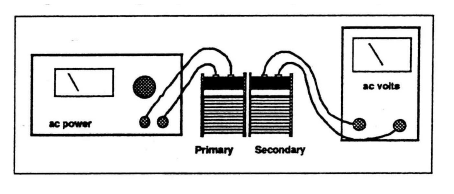
\includegraphics{Esqtransf.png}
    \caption{Esquema del circuit per l'estudi simplificat}
    \label{fig:esq1}
\end{figure}

Com s'explica a la secció \cref{sec:introducció}, per un transformador real l'equació \cref{eq:transf1} no es compleix. L'expressió que descriu la situació en aquest cas és la següent:

\begin{equation}\label{eq:transf2}
     k\frac{V_1}{V_2}=\frac{n_1}{n_2}
\end{equation}

On $k$ és una constant adimensional que es troba entre $0$ i $1$, que és una espècie de mesura del flux que indueix el corrent respecte el total. En el cas del transformador ideal $k=1$.Per tant, per diferents configuracions del transformador i diferents bobines, s'estudiaran els diferents valors de la constant $k$, fent ús de l'equació \cref{eq:transf2}.

\subsection{Estudi com a circuit}\label{sec:metcirc}

En la segona part s'estudia com ja hem dit el transformador com a circuit. Totes les mesures d'aquest apartat són fetes amb el circuit com mostra la figura \cref{fig:esq2}, i com la mateixa figura mostra, en aquest cas, es connecta una resistència al circuit secundari. Per a aquest circuit, emprant les lleis de Kirchh
off s'obtenen certes solucions per les relacions dels voltatges i intensitats d'entrada i sortida. 

\begin{figure}[htbp!]
    \centering \small \sffamily
    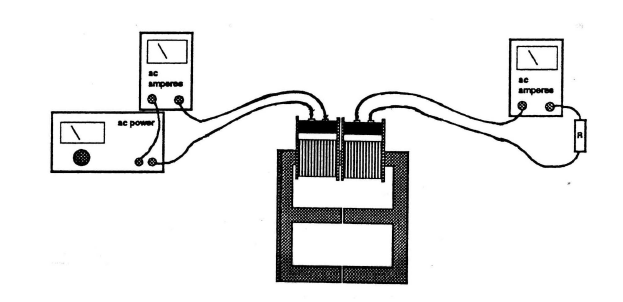
\includegraphics{esqtransf2.png}
    \caption{Esquema del circuit per l'estudi com a circuit amb impedància}
    \label{fig:esq2}
\end{figure}

Inicialment amb una resistència de $R=\SI{1000}{\Omega}$ s'estudien les grans variacions d'intensitat en el circuit primari, només canviant la configuració del transformador. 

Posteriorment, per les bobines de $400$ i $800$ voltes en el primari i amb el circuit obert a la sortida del transformador, es mesura  la intensitat del primari $I_1$, el voltatge del primari $V_1$ i es calcula la reactància $X$ de la bobina segons :

\begin{equation}\label{eq:reac}
    X=\frac{|V_1|}{|I_1|}
\end{equation}

L'equació \cref{eq:reac} s'obté de l'aproximació en el cas que la impedància $Z$ compleix que $Z \gg X$ . Aquest és el nostre cas ja que al tenir el circuit obert la impedància $Z$ es pot considerar infinita. 

Finalment amb les resistències de $R=\SI{1000}{\Omega}$, $R=\SI{100}{\Omega}$ , $R=\SI{10}{\Omega}$ i amb $V_1=\SI{6}{V}$; es mesuren $V_2$, $I_2$ i $I_1$. En els tres casos amb bobines de $400$ voltes, tant al primari com al secundari. Després es repeteix el procediment amb la bobina de $800$ voltes al secundari.


\section{Presentació dels resultats}
\subsection{Estudi simplificat}

Com s'ha comentat a la secció \cref{sec:met} s'ha estudiat el comportament de $k$ per cadascuna de les configuracions del transformador de la figura \cref{fig:transfs}.
A més, també s'ha estudiat el cas en què no hi havia nucli de ferro a l'interior de les bobines (l'anomenarem $0$). Tot això s'ha fet amb $V_1=\SI{6}{V}$ i amb bobines de $400$ al primari i al secundari.

\begin{figure}
    \centering \small \sffamily
    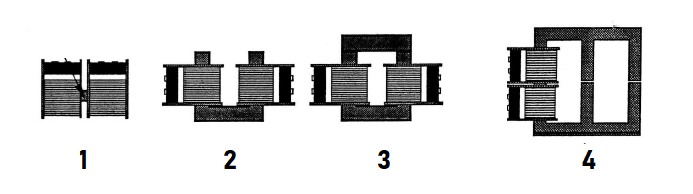
\includegraphics{Transfs.png}
    \caption{Diferents configuracions del transformador}
    \label{fig:transfs}
\end{figure}

Així pels cinc casos s'ha obtingut un voltatge de sortida $V_2$ i una $k$. A més, pel cas amb millor voltatge de sortida, s'ha estudiat també la variació de $k$ per les diferents combinacions de bobines.

 \begin{table}[!htbp]
     \centering
     \caption{Valors de $k$ i $V_2$ per les diferents configuracions}
     \label{tab:k}
\begin{tabular}{SSS}
			\toprule
			{Configuració} & { $k$ \SI{d2}{}} & {$V_2$ (\si{V})}  \\
			\midrule
			0 &  4.17 $\pm$ 0.17 & 0.25 $\pm$ 0.01 \\
			1 & 45.13 $\pm$ 0.67 & 2.71 $\pm$ 0.04 \\
			2 & 35.88 $\pm$ 0.50 & 2.15 $\pm$ 0.03 \\
			3 & 89.13 $\pm$ 0.83 & 5.35 $\pm$ 0.05 \\
			4 & 97.46 $\pm$ 0.83 & 5.85 $\pm$ 0.05 \\
			\bottomrule
\end{tabular}
\end{table}

Els resultats comproven que la configuració més eficaç és la número $4$. Els diferents valors de $k$ semblen indicar que hi ha dos fets determinants a l'hora d'augmentar el rendiment del transformador. Primerament el fet que les dues bobines es trobin molt properes l'una a l'altra sembla augmentar considerablement el rendiment, cosa que és lògica d'esperar ja que el flux passarà en més quantitat per la bobina del secundari. A més d'això, el fet que el nucli de ferro segueixi la trajectòria de les línies de camp, també augmenta el rendiment; aquest fet també és d'esperar ja que al ser el ferro un material ferromagnètic condueix bé el flux magnètic a través de l'espai optimitzant-ne l'arribada a l'altra bobina. Evidentment al ser la configuració $4$ la de major potencial de sortida, l'estudi de les diferents bobines ha estat fet amb aquesta.

 \begin{table}[!htbp]\textwidth
     \centering
     \setlength\tabcolsep{2pt}
     \caption{Valors de $k \cdot \SI{d2}{}$ per diferents combinacions de bobines a la configuració $4$}
     \label{tab:k4}
\begin{tabular}{p{2cm}p{2,5cm}p{2,5cm}p{2,5cm}p{2,5cm}p{2,5cm}}
			\toprule
		   {Sec.|Prim.}    &200&400&800&1600&3200 \\
			\midrule
			200 &  & 96.62 $\pm$ 0.34  & 95.33 $\pm$ 0.67 & 94.00 $\pm$ 0.27 &  93.93 $\pm$ 0.27 \\
			400 &  99.58 $\pm$ 0.50 & 95.60 $\pm$ 0.68 & 95.58 $\pm$ 0.67 & 96.33 $\pm$ 0.27 & 94.17 $\pm$ 0.27 \\
			800 &  97.81 $\pm$ 0.38 & 97.08 $\pm$ 0.51 & & 95.00 $\pm$ 0.67 & 92.47 $\pm$ 0.33\\
			1600 &  97.45 $\pm$ 0.16 & 97.50 $\pm$ 0.34 & 94.58 $\pm$ 0.33 & & 92.50 $\pm$ 0.67\\
			3200 & 98.70 $\pm$ 0.19 & 97.72 $\pm$ 0.19 & 94.58 $\pm$ 0.29 & 95.50 $\pm$ 0.33 & \\
			\bottomrule
\end{tabular}
\end{table}

La taula \cref{tab:k4} sembla indicar que per a més voltes a la bobina principal $ k$ disminueix. Aquest fet podria ser explicat pensant que el flux total generat per les bobines de més voltes és major i, per tant,  possiblement és més complicat que aquest travessi comoletament la segona bobina. A més la bobina que sembla funcionar millor en el secundari és la de $400$, exceptuant el cas en què la del primari també és $400$. Tanmateix, les diferències són molt petites i l'estudi no ha estat suficientment exhaustiu com per concloure que la bobina de $400$ sempre serà la més eficaç en el secundari.

\subsection{Estudi com a circuit}

Com s'ha comentat, primerament s'han mesurat les intensitats del primari per diferents configuracions i s'ha analitzat les variacions. Aquestes mesures han estat realitzades amb la bobina de $800$ al primari i la de $400$ al secundari, amb un potencial d'entrada de $V=\SI{6}{V}$ i amb una impedància $Z=\SI{1000}{\Omega}$. 

 \begin{table}[!htbp]
     \centering
     \caption{Valors de $I_1$ i $k \SI{d2}{}$ per les diferents configuracions}
     \label{tab:I1}
\begin{tabular}{SSS}
			\toprule
			{Configuració} & { \approx $k$ \SI{d2}{}} & {$I_1$ (\si{A})}  \\
			\midrule
			0 &  4.17 $\pm$ 0.17 & 0.56 $\pm$ 0.04 \\
			1 & 45.13 $\pm$ 0.67 & 0.29 $\pm$ 0.03 \\
			2 & 35.88 $\pm$ 0.50 & 0.15 $\pm$ 0.02 \\
			3 & 89.13 $\pm$ 0.83 & 0.034 $\pm$ 0.001 \\
			4 & 95.58 $\pm$ 0.67 & 0.018 $\pm$ 0.001 \\
			\bottomrule
\end{tabular}
\end{table}

Amb la informació de la taula \cref{tab:I1} es veu que $I_1$ varia considerablement amb les diferents configuracions.  Aquesta variació es pot explicar amb la variació de $k$. Per les configuracions amb major $k$ el flux que travessa la bobina secundària augmenta i, per tant, també ho fa el flux de la secundària que travessa la primària. Aquest segon flux crea una força contraelectromotriu que disminueix el potencial al primari i per tant $I_1$.
\newline
\\

Pel que fa a la reactància del circuit, com s'ha comentat a la seccio \cref{sec:metcirc}, es pot calcular la reactància segons l'equació \cref{eq:reac}. Per la bobina de $400$ els valors obtinguts han estat $I_{1,400}=(54.33 \pm 0.10) \si{mA}$ i $X_{400}=(110.45 \pm 1.8)\si{\Omega}$. Per la bobina de $800$ els valors han estat $I_{1,800}=(18.55 \pm 0.10) \si{mA}$ i $X_{800}=(323.45 \pm 5.4)\si{\Omega}$.

Obviament al tenir menor intensitat la bobina de $800$ voltes, amb el mateix voltatge que la de $400$, això implicarà una major impedància per la de $800$ que és el resultat calculat.
\newline
\\

Finalment s'han calculat $I_1$, $I_2$ i $V_2$ per la configuració amb $400$ voltes tant al primari com al secundari, amb les resistències de $1000\si{\Omega}$, $100\si{\Omega}$ i $10\si{\Omega}$.

 \begin{table}[!htbp]
     \centering
     \caption{Valors de $I_1$ i $I_2$ i $V_2$ per $400$ voltes en el primari i en el secundari}
     \label{tab:400IV}
\begin{tabular}{SSSSSS}
			\toprule
			{Z (\si{\Omega})} & { $I_1$ (\si{mA})} & {$I_2$ (\si{mA})} &  {$V_2$ (\si{V})} & { $\frac{V_2}{V_1}_{exp}$} & { $\frac{V_2}{V_1}_{teo}$}   \\
			\midrule
			10 &  320$\pm$1 &  325$\pm$1 & 3.46 $\pm$ 0.1 & 0.58 & 0.69 \\
			100 & 72.2$\pm$0.1 & 42.8$\pm$0.1 & 5.51 $\pm$ 0.01 & 0.92  & 0.96 \\
			1000 & 51.3$\pm$0.1 & 5.3$\pm$0.1 & 5.76 $\pm$ 0.01 & 0.96  & 0.96 \\
			\bottomrule
\end{tabular}
\end{table}

Per la taula \cref{tab:400IV} podem veure que, com era d'esperar, a majors impedàncies les intensitats que circulen per ambdós circuits disminueixen. Pel que fa als valors dels guanys aquests són prou propers als valors teòrics, calculant els percentatges d'error surten de aproximadament el $1\%$, el $4\%$ i el $18\%$ respectivament per les impedàncies de $1000\si{\Omega}$,  $100\si{\Omega}$
 i  $10\si{\Omega}$ . Tanmateix hi ha una variació entre els guanys de $Z=1000\si{\Omega}$ i $Z=100\si{\Omega}$ que no hauria de aparèixer teòricament. Aquest fet probablement és degut a les aproxim
acions a l'hora de trobar les solucions de les equacions de Kirchhoff pel circuit. El fet que  per $Z=10\si{\Omega}$ $V_2$ disminueixi considerablement, és degut a que el terme de la força contraelectromotriu apareix en l'aproximació de $Z\ll X$ i fa disminuir $V_2$. El fet principal que s'observa relatiu a $Z$, és l'augment del guany per a impedàncies $Z$ més elevades.


 \begin{table}[!htbp]
     \centering
     \caption{Valors de $I_1$ i $I_2$ i $V_2$ per $400$ voltes en el primari i  $800$ en el secundari}
     \label{tab:800IV}
\begin{tabular}{SSSSSS}
			\toprule
			{Z (\si{\Omega})} & { $I_1$ (\si{mA})} & {$I_2$ (\si{mA})} &  {$V_2$ (\si{V})} & { $\frac{V_2}{V_1}_{exp}$} & { $\frac{V_2}{V_1}_{teo}$}   \\
			\midrule
			10 &  533 $\pm$1 &  248$\pm$1 & 2.68 $\pm$ 0.01 & 0.45 & 0.32 \\
			100 & 140$\pm$ 1 & 63.8$\pm$0.1 & 9.37 $\pm$ 0.01 & 1.59  & 1.94 \\
			1000 & 552$\pm$ 1 & 10.2$\pm$0.1 & 11.39 $\pm$ 0.01 & 1.90  & 1.94 \\
			\bottomrule
\end{tabular}
\end{table}

A la taula \cref{tab:800IV} es poden observar els mateixos efectes mencionats per la taula \cref{tab:400IV}. En aquest cas, els percentatges de error aproximats són de $2\%$, $18\%$ i $38\%$ respectivament per les impedàncies de $1000\si{\Omega}$,  $100\si{\Omega}$  i  $10\si{\Omega}$, el valor del guany per la resistència de $10\si{\Omega}$ és la que difereix més notablement del valor teòric esperat. Els valors de la taula \cref{tab:800IV}, a més a més, han accentuat en alguns casos els efectes mencionats per la bobina de $400$. Ja que, per exemple, la disminució de $V_2$  per la de $800$ voltes ha estat molt considerable. El valor esperat teòricament era de $V_2=\SI{12}{V}$, en canvi el valor mesurat ha estat de $V_2=(2.68 \pm 0.01) \si{V}$. També podem observar de la relació entre les dues taules que els valors teòrics han canviat considerablement degut al canvi de $k$. 

\section{Conclusions}

Pel que fa al primer estudi del transformador, les conclusions més interessants han estat veure que sembla que $k$, i per tant l'eficiència del circuit, és major per configuracions amb bobines de menys voltes al primari. El nucli de ferro també augmenta en gran mesura $k$, i el fet que aquest segueixi la forma de les línies de camp magnètic també sembla ajudar a augmentar $k$. A més de tots aquests factors, la proximitat de la bobina també sembla ser un factor rellevant, essent més eficients els transformadors amb les bobines més properes.
\newline

Per la segona part de l'estudi, s'ha observat que només variant la configuració del transformador ja varia en gran mesura la intensitat de sortida $I_1$. Les configuracions de major $k$ han resultat ser les de menor $I_1$. A més el guany de voltatge $\frac{V_2}{V_1}$ resulta ser major per circuits amb impedàncies $Z$ més elevades. Finalment, també s'ha observat que el voltatge en el circuit secundari disminueix considerablement si la impedància $Z$ del circuit també ho fa.